\documentclass{standalone}
\usepackage{tikz}
\usepackage{amsmath}
\usetikzlibrary{shapes.geometric, backgrounds}

\begin{document}
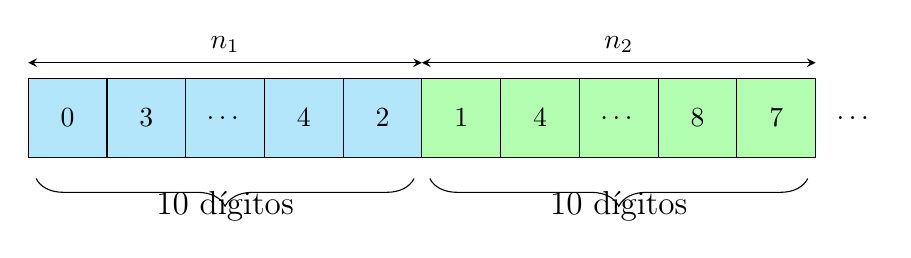
\begin{tikzpicture}

    % Dibuja las celdas con los dígitos y rellena las celdas con diferentes colores
    \foreach \x/\val in {0/0, 1/3, 2/\ldots, 3/4, 4/2, 5/1, 6/4, 7/\ldots, 8/8, 9/7} {
        % Rellena las primeras 5 celdas con un color (por ejemplo, azul claro)
        \ifnum\x<5
            \filldraw[fill=cyan!30] (\x,0) rectangle ++(1,1);
        \else
            % Rellena las siguientes celdas con otro color (por ejemplo, verde claro)
            \filldraw[fill=green!30] (\x,0) rectangle ++(1,1);
        \fi
        \node at (\x+0.5,0.5) {\val};
    }
    
    % Puntos suspensivos antes y después de las celdas
    \node at (10.5,0.5) {\ldots};

    % Corchetes para grupos de dígitos
    \draw[decorate,decoration={brace,amplitude=10pt,mirror,raise=2pt},yshift=0pt] (0.1,-0.2) -- (4.9,-0.2) node [black,midway,yshift=-12pt] {\large 10 dígitos};
    \draw[decorate,decoration={brace,amplitude=10pt,mirror,raise=2pt},yshift=0pt] (5.1,-0.2) -- (9.9,-0.2) node [black,midway,yshift=-12pt] {\large 10 dígitos};

    % Marcas de los intervalos N1, N2, N3
    \draw [stealth-stealth] (0,1.2) -- (5,1.2) node[midway, above] {$n_1$};
    \draw [stealth-stealth] (5,1.2) -- (10,1.2) node[midway, above] {$n_2$};

\end{tikzpicture}
\end{document}
